%%%%%%%%%%%%%%%%%%%%%%%%%%%%%%%%%%%%%%%%%%%%%%%%%%%%%%%%%%%%%%%%%%%%%%%%%%%%%%%
% ------------------- Mathematical Logbook - by Jonas Frede -------------------
%%%%%%%%%%%%%%%%%%%%%%%%%%%%%%%%%%%%%%%%%%%%%%%%%%%%%%%%%%%%%%%%%%%%%%%%%%%%%%%
%
% NOTE: This document can switch between printing and on-screen version.
% NOTE: Also, english and german versions are available.
%
%------------------------------------------------------------------------------
% DOCUMENT CLASS AND INCLUDED CONFIGURATIONS
%------------------------------------------------------------------------------

\documentclass[% NOTE: Switch between a5paper and a4paper here
a4paper,11pt, % The default document font size, options: 10pt, 11pt, 12pt
oneside, % Two side (alternating margins) for binding by default, uncomment to switch to one side
english, ngerman, % Babel: English, of course, and ngerman for German (duh)
onehalfspacing, % singlespacing, alternatives: onehalfspacing or doublespacing
%draft, % Uncomment to enable draft mode (no pictures, no links, overfull hboxes indicated)
%nolistspacing, % If the document is onehalfspacing or doublespacing, uncomment this to set spacing in lists to single
%liststotoc, % Uncomment to add the list of figures/tables/etc to the table of contents
%toctotoc, % Uncomment to add the main table of contents to the table of contents
parskip=half-, % Add space between paragraphs, allows for multiple parameters
%nohyperref, % Uncomment to not load the hyperref package
%headsepline, % Uncomment to get a line under the header
%footsepline, % Uncomment to get a line over the footer
chapterinoneline, % Uncomment to place the chapter title next to the number on one line
numbers=noenddot, % Uncomment for Definition 2.3 instead of 2.3.
%dvipsnames, % xcolor parameter
]{studybook}

%\parfillskip=0pt % All paragraphs become rectangles, just for the lulz, usually throws many warnings

%------------------------------------------------------------------------------
% ENCODINGS AND FONT PACKAGES
%------------------------------------------------------------------------------

\usepackage[T1]{fontenc} % Encoding in PDF
\usepackage[utf8]{inputenx} % UTF8-encoding in source file
\usepackage{fourier} % Main font package!
%\usepackage{fontawesome} % For nice symbols
\usepackage{bm} % Bold math symbols (must be loaded after fonts)

%------------------------------------------------------------------------------
% BIBLIOGRAPHY, INDEX AND CITATIONS
%------------------------------------------------------------------------------

\usepackage[hyperref, backref, backend=biber, bibencoding=utf8, style=numeric, sorting=nty, sortcites=true]{biblatex}
\usepackage[autostyle=true]{csquotes}
\usepackage{makeidx}

\addbibresource{logreferences.bib}
\makeindex

%------------------------------------------------------------------------------
% GENERAL INFORMATION
%------------------------------------------------------------------------------

\documenttitle{\IfLanguageName{english}{A Mathematician's Logbook}{Logbuch eines Mathematikers}} % The document title, print it elsewhere with \doctitle
\author{Jonas Frede} % Your name, print it elsewhere with \authorname
\keywords{mathematics} % Keywords, print it elsewhere with \keywordnames

\AtBeginDocument{
\hypersetup{english}
\hypersetup{pdftitle=\doctitle} % Set the PDF's title to your title
\hypersetup{pdfauthor=\authorname} % Set the PDF's author to your name
\hypersetup{pdfkeywords=\keywordnames} % Set the PDF's keywords to your keywords
}

\usepackage{preamble} % all custom commands go here TODO: split this file!

%------------------------------------------------------------------------------
% MARGIN AND TYPOGRAPHY LAYOUT SETTINGS
%------------------------------------------------------------------------------

% uncomment to show how the textframe is set on the page
%\geometry{showframe}

\widegeometry % NOTE: Change page margins between onscreengeometry (a5paper) and widegeometry (a4paper)

\usepackage[%
activate={true,nocompatibility}, % activate={true,nocompatibility} - activate protrusion and expansion
final, % final - enable microtype; use "draft" to disable
tracking=true, % tracking=true, kerning=true, spacing=true - activate these techniques
kerning=true, %
spacing=true, %
factor=1100, % add 10% to the protrusion amount (default is 1000)
stretch=10, %
shrink=10 % reduce stretchability/shrinkability (default is 20/20)
]{microtype}

%------------------------------------------------------------------------------
% DOCUMENT START AND LANGUAGE SELECTION
%------------------------------------------------------------------------------

\begin{document}
\frontmatter % Use roman page numbering style (i, ii, iii, iv...) for the pre-content pages
\pagestyle{empty} % Default to the empty heading style until the book style is called for the body content

\selectlanguage{english} % NOTE: Select the displayed language

%------------------------------------------------------------------------------
% TITLE PAGE
%------------------------------------------------------------------------------

\begin{titlepage}
\begin{center}

% Spacing
\vspace*{.06\textheight}
%\vspace{1cm}
\mbox{}\\[0.1cm]

\thinRule\par% Horizontal line
{\fontsize{40pt}{36pt}\scshape\doctitle\par} % Title
\par\thinRule% Horizontal line

\vfill

\begin{minipage}[t]{0.5\textwidth}
\begin{center} \large
\emph{\IfLanguageName{english}{Author}{Autor}:}\\
{\authorname}
\end{center}
\end{minipage}\\[1.5cm]

\vfill

\large\textit{\IfLanguageName{english}{A document written in LaTeX}{Ein Dokument, geschrieben in LaTeX} \\ \IfLanguageName{english}{containing a selection of topics}{enthält eine Auswahl an Themen} \\ \IfLanguageName{english}{to study for a mathematics degree}{zum Studium der Mathematik}}\\[1cm]
\textit{\IfLanguageName{english}{created for students and interested parties}{für Studenten und Interessierte}}\\[2cm]

\vfill

\IfLanguageName{english}{English version of \today}{Deutsche Version vom \today}\\[3cm] % Date, uses iflang switch

\vfill
\end{center}
\end{titlepage}

%------------------------------------------------------------------------------
% LIST OF CONTENTS/FIGURES/TABLES PAGES
%------------------------------------------------------------------------------

\pagestyle{plain}
\setcounter{page}{0} % next page will be page I
\pagenumbering{Roman} % big roman numbering

% INTRODUCTION - BY Jonas Frede
% !TEX root = ../MathLog.tex

\chapter*{\IfLanguageName{english}{Preface}{Vorwort}}

\IfLanguageName{english}{\todonote{translate here}}{Im Internet stieß ich auf einen Beitrag einer Person, welche ein Logbuch führt, in dem sie mathematische Fakten, Ideen und Gelerntes festhält. Daraus erwuchs für mich das Bedürfnis, neben neu erlerntem Stoff auch gelernte Dinge zu wiederholen, indem ich alte Mitschriften meiner Vorlesungen digitalisiere und mit eigenen Kommentaren erweitere.

Dieses Dokument soll dem oben genannten Zweck dienen, und wird daher Gegenstand ständiger Veränderung und Erweiterung sein. Das Datum der letzten Änderung findet sich auf der Titelseite.

Eventuell können Teile dieses Projektes auch für andere Menschen von Nutzen sein. Daher wird oft in einem einladenden und in der Mathematik üblichen Ton von \enquote{wir} gesprochen. Ich freue mich über Hinweise auf Fehler und Tipps, da ich keinesfalls vorgeben möchte, in allen vorgestellten Bereichen ein Experte zu sein. Viel Spaß beim Lesen!}

\mbox{}\newline
  \hspace*{\fill} \IfLanguageName{english}{Berlin, January 25th, 2017}{Berlin, den 25.01.2017} \\
  \hspace*{\fill} Jonas Frede

\newpage
\section*{\IfLanguageName{english}{Recommendation for the reader}{Empfehlung für den Leser}}
\IfLanguageName{english}{\todonote{translate here}}{Natürlich kann man als interessierter Leser wie Sie dort einsteigen, wo man möchte. Jemandem, der ein wenig Anleitung haben möchte, empfehle ich folgendes Diagramm, in welcher Reihenfolge eine Lektüre empfehlenswert ist:}

\todowarning{diagram for order of chapters to read}

\IfLanguageName{english}{\todonote{translate here}}{Der unerfahrene und lernende Leser sei dazu angehalten, die im Text getätigten Aussagen zu verifizieren. Der Inhalt mag anfangs einfach und offensichtlich wirken, allerdings ist empfohlen, die Art und Form der Wissensvermittlung zu berücksichtigen, da diese besonders wichtig ist und der Mathematik eigen ist: Aussagen (wie ein \emph{Satz, Lemma} oder ähnliches) müssen grundsätzlich auf bereits bekanntes Wissen und vorher bekannte Aussagen logisch zurückgeführt werden, mit Hilfe eines \emph{Beweises}.
Man sollte daher versuchen, jede Aussage und jeden Beweisschritt nachzuvollziehen und, falls möglich, mitzuschreiben. Nicht zuletzt, um die Lesegeschwindigkeit zu drosseln. Fügen Sie Details, die ihrer Meinung nach im Text fehlen, ein, und teilen Sie mir gerne Verbesserungsvorschläge mit.

Fragen, die beim Lesen des Textes an verschiedenen Stellen helfen sollen, sind beispielsweise \enquote{Kann ich die Definition oder den Satz in eigenen Worten wiedergeben?}, \enquote{Kenne ich ein Beispiel für die beschriebene Definition oder Voraussetzung?} und \enquote{Kenne ich ein Beispiel, für das die Voraussetzungen einer Aussage nicht erfüllt sind?}.
Zu Sätzen sollte man sich zusätzlich fragen \enquote{Was sind die Voraussetzungen, was ist die Behauptung?}, und bevor man einen Beweis beginnt zu lesen, ist es hilfreich, sich zuerst selbst die Frage zu beantworten \enquote{Was ist in einem Beweis zu tun, um aus den Voraussetzungen die Behauptung herzuleiten?}.
In der Erarbeitung eines Beweises der Form \enquote{Aus \(A\) folgt \(B\)} ist es schließlich wichtig, sich zu fragen \enquote{Habe ich verstanden, warum \(B\) aus \(A\) folgt?}.

Für eine etwas ausführlichere Einführung in das mathematische Arbeiten sei auf das lehrreiche Skript und Buch~\cite{SchicS:Einfuehrungindas} und dessen Quellen verwiesen.}


\tableofcontents%
\listoffixmes%

%------------------------------------------------------------------------------
% CONTENT - CHAPTERS
%------------------------------------------------------------------------------

\mainmatter % Begin numeric (1,2,3...) page numbering
\pagestyle{book} % Return the page headers back to the main style

% Include the chapters as separate files inside the grouping files below
% !TEX root = ../MathLog.tex

% !TEX root = ../../MathLog.tex

\chapter{\IfLanguageName{english}{Foundations of Mathematics}{Grundlagen der Mathematik}}

\IfLanguageName{english}{\todonote{translate introductory paragraph}}{Wo beginnt man am Besten mit den Grundlagen in der Mathematik? Ich denke, es ist sinnvoll, sich klar zu machen, dass die Grenze zwischen Grundlagen und fortgeschrittenem Material oftmals nicht klar gezogen werden kann. Allerdings möchte ich es trotzdem wagen, ein paar Themen als Grundlagen vorzustellen, um auf diesem Fundament weitere Bereiche der Mathematik zu entdecken und zu erarbeiten.}

\section{\IfLanguageName{english}{Elements of Logic}{Elemente der Logik}}

\IfLanguageName{english}{\todonote{translate everything here}}{Ein Thema, welches man wohl in jedem Fall am Anfang erwähnen möchte, weil sie das täglich Brot eines Mathematikers oder Mathematikstudenten bilden, sind \emph{logische Aussagen}. Eine logische Aussage ist ein Satz, der einen eindeutigen \emph{Wahrheitswert} besitzt, also entweder wahr oder falsch ist (wir nutzen das Prinzip des ausgeschlossenen Dritten, lat. tertium non datur):

\begin{example}
  Der Satz \enquote{1 ist eine positive Zahl} ist wahr, wohingegen \enquote{2 ist eine negative Zahl} oder \enquote{Der Mond ist aus Käse} falsch ist. Alle drei Sätze sind also logische Aussagen. Je nach Wetterlage hat die Aussage \enquote{Die Sonne scheint.} einen eindeutig bestimmten Wahrheitsgehalt, ist also ebenfalls eine logische Aussage. \enquote{Hallo!} oder \enquote{Möchtest du etwas essen?} sind keine logischen Aussagen, da ihnen kein Wahrheitsgehalt sinnvoll zugeordnet werden kann.
\end{example}

Das Beispiel des Wetters zeigt bereits, dass der Wahrheitsgehalt einer Aussage vom Kontext abhängig sein kann. In der Mathematik versucht man daher, den Kontext möglichst klar zu formulieren und daher alle Aussagen, die man trifft, auf einige wenige Grundannahmen zurück zu führen, die man als wahr annehmen muss. Diese Grundannahmen nennt man \emph{Axiome}. Man könnte beispielsweise das Prinzip des ausgeschlossenen Dritten als Axiom verstehen. Eine genauere und tiefere Betrachtung von Axiomen verschieben wir jedoch auf ein späteres Kapitel.

Eine wichtige Erweiterung logischer Aussagen sind so genannte \emph{Aussageformen}. Dies sind Aussagen, die eine oder mehrere freie Variablen enthalten, zum Beispiel \enquote{$x$ ist eine negative Zahl}. Der Wahrheitswert kann im Allgemeinen erst dann ermittelt werden, wenn die Variablen durch Konstanten ersetzt wurden: Für $x=-10$ ist die Aussage wahr, für $x=1$ ist sie falsch. Es gibt allerdings Aussageformen, die immer wahr beziehungsweise falsch sind: ein Beispiel wäre \enquote{Es ist entweder $x$ eine Zahl oder keine Zahl.}

Weiterhin möchten wir Aussagen mit \emph{Quantifizierungen} betrachten, welche die wohl häufigste Art von logischen Aussagen im mathematischen Gebrauch sind.

\begin{example}
  Eine Aussage wie \enquote{Es gibt eine reelle Zahl $x$, so dass $x^2 \leq 2$} ist eine Existenzaussage,
  eine Aussage wie \enquote{Für alle positiven reellen Zahlen $x$ gilt $x^2 \leq 1$} ist eine Allaussage.
\end{example}

Der \emph{Quantor} \enquote{Es gibt} wird mit $\exists$ abgekürzt, der Quantor \enquote{Für alle} mit $\forall$.

\begin{example}[fortgesetzt]
  Die erste Aussage oben lässt sich schreiben als \enquote{$\exists x \in \RR$, s.d. $x^2 \leq 2$}, die zweite Aussage als \enquote{$\forall x \in \RR_{>0}$ ist $x^2 \leq 1$}.
\end{example}

Aussagen mit Quantifizierungen haben wieder nur einen Wahrheitswert. Die erste Aussage des Beispiels ist wahr, die zweite falsch. Da wir nun im Vorgriff bereits ein paar Mengen genutzt haben, die wir eigentlich noch nicht wirklich kennen, wollen wir diese zuerst einmal nur über ihre Notation einführen:

\begin{notation}[Ein paar Mengen]
  \mbox{}
  \begin{itemize}
    \item $\RR$ sind die reellen Zahlen. Diese wollen wir später noch genauer charakterisieren.
    \item $\ZZ$ sind die ganzen Zahlen $\{\ldots,-2,-1,0,1,2,\ldots\}$.
    \item $\NN$ sind die natürlichen Zahlen $\{1,2,3,\ldots\}$, $\NN_0$ ist $\{0,1,2,3,\ldots\}$.
    \item $\QQ$ sind die rationalen Zahlen \(\setdef{\frac{p}{q}}[p \in \ZZ, q \in \NN]\).
  \end{itemize}
\end{notation}

% Aussonderungsaxiom - Axiomenschema (s.u.)
% Aussagenkalkül, Wahrheitstafeln, logische Operatoren
% notwendig & hinreichend !!!

\section{Mengen}

% Mengenkram, Operatoren und so.

\section{Axiomatische Mengenlehre}

Unsere bisher naive Behandlung von Mengen soll hier durch ein grundlegendes Axiomensystem fundiert werden, welches 1930 von \textcite{Zerme:UeberGrenzzahlenund} eingeführt wurde. Das Axiomensystem wird daher auch als ZF(-System) bezeichnet. Oftmals möchte man ebenfalls das so genannte Auswahlaxiom (Axiom of Choice) zu diesem System hinzufügen, dann nennt man das System auch ZFC.}


\part{\IfLanguageName{english}{Algebra and Number Theory}{Algebra und Zahlentheorie}}

% !TEX root = ../../MathLog.tex
\chapter{\IfLanguageName{english}{Linear Algebra}{Lineare Algebra}}

% !TEX root = ../../MathLog.tex

\chapter{Algebra}

\IfLanguageName{english}{\todonote{translate here}}{Die Algebra in ihrer abstrakten Form ist ein Teilgebiet der Mathematik, das sich mit algebraischen Strukturen befasst. Im Gegensatz zur linearen Algebra, welche oft den ersten Kontakt mit algebraischen Strukturen darstellt, wollen wir die abstrakte Algebra ein wenig allgemeiner halten, aber trotzdem mit schönen Beispielen anreichern.

Methoden der Algebra finden Anwendung in fast allen anderen Bereichen der Mathematik und bringen selbst wieder neue Bereiche hervor, wie beispielsweise die Darstellungs- oder Kategorientheorie. Ein sinnvolles Ziel für einen ersten Kurs in Algebra bildet die Aussage, dass die allgemeine Nullstellengleichung eines Polynoms fünften Grades im Gegensatz zu denen kleineren Grades nicht durch Formeln lösbar ist.

\section{Gruppentheorie}

Der erste Teil einer grundlegenden Algebra bildet die Beschäftigung mit Gruppen und ihren Verwandten:

\begin{definition}[Monoid]
  Eine Menge $M$ mit einer Abbildung $\cdot \colon M \times M \rightarrow M$ heißt \emph{Monoid}, falls:
  \begin{enumerate}
    \item $(a \cdot b) \cdot c = a \cdot (b \cdot c)$ für alle $a,b,c \in M$, also $\cdot$ assoziativ.
    \item Es gibt ein $e \in M$, so dass $e \cdot a = a \cdot e = a$ für alle $a \in M$ (ein neutrales Element).
  \end{enumerate}
\end{definition}

Die Abbildung $\cdot$ nennt man auch eine zweistellige Verknüpfung auf $M$. Ist $(M,\cdot)$ nun ein Monoid, so kann man für endlich viele Elemente $a_1, \ldots, a_n \in M$ das \emph{Produkt}:
\[
  \prod_{i=1}^{n} a_i \coloneqq a_1 \cdot \ldots \cdot a_n
\]
definieren, sowie für jedes $a \in M$ und $n \in \NN$ die $n$-te \emph{Potenz} von $a$, mittels:
\[
  a^n \coloneqq \prod_{i=1}^{n} a, \> \mathrm{sowie} \> a^0 = e.
\]

Ein Monoid ist die einfachste algebraische Struktur, die uns zu diesem Zeitpunkt interessieren soll. Lassen wir die Existenz des neutralen Elements fallen, so bildet die dadurch definierte Struktur eine \emph{Halbgruppe}. Lassen wir zusätzlich die Assoziativität weg, so bezeichnen wir $(M,\cdot)$ als \emph{Magma}. Indem wir von einem Monoid nun noch eine weitere Eigenschaft fordern, gelangen wir zum Hauptbegriff dieses Abschnittes:

\begin{definition}[Gruppe]
  Eine Menge $G$ mit einer Abbildung $\cdot \colon G \times G \rightarrow G$ heißt \emph{Gruppe}, falls $(G,\cdot)$ ein Monoid ist, und zusätzlich gilt:
  \begin{enumerate}\setcounter{enumi}{2}
    \item Zu jedem Element $a \in G$ gibt es ein so genanntes \emph{inverses} Element $b \in G$, das heißt: $a \cdot b = b \cdot a = e$.
  \end{enumerate}
  $G$ heißt \emph{kommutativ} oder \emph{abelsch}, falls zusätzlich gilt:
  \begin{enumerate}\setcounter{enumi}{3}
    \item Für alle $a,c \in G$ gilt $a \cdot c = c \cdot a$.
  \end{enumerate}
\end{definition}

Für eine kürzere Schreibweise entscheiden wir uns hier für folgende Notation:

\begin{notation}
  Wir schreiben: $(G,\cdot)$ ist eine Gruppe. Falls die Abbildung $\cdot$ klar ist, schreiben wir nur $G$ für eine Gruppe, und $a \cdot b$ schreiben wir dann nur noch als $ab$.
\end{notation}

Zuerst wollen wir festhalten, dass aus den bisherigen Definitionen bereits zwei fundamentale Charakteristika von Monoiden und Gruppen ableitbar sind:

\begin{proposition}[Eindeutigkeit von neutralen und inversen Elementen]
  Sei $M$ ein Monoid und $G$ eine Gruppe.
  \begin{enumerate}
    \item $M$ (und damit auch jede Gruppe) hat ein eindeutiges neutrales Element.
    \item Jedes Element $a \in G$ hat ein eindeutiges inverses Element.
  \end{enumerate}
\end{proposition}

\begin{proof}
  \begin{enumerate}
    \item Sind $e,e' \in M$ zwei neutrale Elemente, so gilt $e = e \cdot e' = e'$, aufgrund der Definition neutraler Elemente.
    \item Seien $b,b' \in G$ Inverse für $a \in G$. Dann gilt $b' = b' \cdot e = b' \cdot (a \cdot b) = (b' \cdot a) \cdot b = e \cdot b = b$, was ebenfalls aus der Definition folgt.
  \end{enumerate}
\end{proof}

In Zukunft können wir also von \textit{dem} neutralen und inversen Element sprechen. Um einen weiteren Bezug zu uns bekannten Objekten herzustellen, führen wir ein wenig zusätzliche Notation ein.

\begin{notation}[Multiplikative und additive Form]
Sei $(G,\cdot)$ eine Gruppe. Das neutrale Element bezüglich $\cdot$ bezeichnet man oft mit $1$. Das Inverse von $a \in G$ wird dann mit $a^{-1}$ bezeichnet. Dies nennt man die \emph{multiplikative Schreibweise} oder \emph{Form} einer Gruppe.
Die Verknüpfung einer abelschen Gruppe schreibt man oft in \emph{additiver Form}, also $a+b$, $\sum_{i=1}^n a_i$, $n \cdot a = \sum_{i=1}^n a$ bezüglich der Definitionen von vorher. Dann bezeichnet man das neutrale Element mit $0$ und das Inverse von $a \in G$ mit $-a$.
\end{notation}

Wir kennen bereits viele Beispiele für Monoide und Gruppen, die diese Notation nutzen, allerdings werden wir nicht jedes Beispiel beweisen und zusätzlich einige Aussagen als Übungsaufgaben stellen.

\begin{example}[Monoide und Gruppen]
  \leavevmode \vspace{-\baselineskip}
  \begin{enumerate}
    \item $(\ZZ,+)$, $(\QQ,+)$, $(\RR,+)$, $(\CC,+)$ sind abelsche Gruppen.
    \item $(\ZZ,\cdot)$, $(\NN,\cdot)$ sind Monoide, aber keine Gruppen.
    \item $(\QQ,\cdot)$ ist keine Gruppe, denn $0$ hat kein Inverses, allerdings ist $(\QQ^*,\cdot)$ eine Gruppe, wobei $\QQ^* \coloneqq \QQ \setminus \setdef{0}$ ist.
    \item Sei $X$ eine Menge und $(G,\cdot)$ eine Gruppe. Sei $\Abb(X,G)$ die Menge aller Abbildungen von $X$ nach $G$. Definiere $* \colon \Abb(X,G) \times \Abb(X,G) \rightarrow \Abb(X,G)$ durch $(f * g)(x) = f(x) \cdot g(x)$ für jedes $x \in X$.
    Dann bildet $(\Abb(X,G),*)$ eine Gruppe mit dem neutralen Element $e \colon X \rightarrow G$, $e(x) = 1$ für $x \in X$ (hier ist $1 \in G$ das neutrale Element von G). Das Inverse von $f \in \Abb(X,G)$ ist $f^{-1}$ mit $f^{-1}(x) = f(x)^{-1}$.
    \item Sei $\KK$ ein Körper und $\KK^\nn$ die Menge der $\nn$-Matrizen über $\KK$, wobei $n \in \NN$ ist. Dann ist $(\KK^\nn,+)$ eine abelsche Gruppe.
    \item Sei $\GL(n,\KK) \coloneqq \left\{ A \in \KK^\nn \suchthat \det(A) \neq 0 \right\}$ die Menge der invertierbaren $\nn$-Matrizen über $\KK$. Dann ist $(\GL(n,\KK),\cdot)$ eine Gruppe mit der Matrixmultiplikation $\cdot$. Diese Gruppe ist nicht abelsch für $n \geq 2$, dies ist eine Übungsaufgabe.
  \end{enumerate}
\end{example}

Die Abkürzung $\GL$ steht für die \enquote{general linear group}, die allgemeine lineare Gruppe, die diesen Namen trägt, weil $\GL(n,\KK)$ in isomorph ist zur Gruppe der linearen Automorphismen auf $\KK^n$.

\subsection{Untergruppen}

\begin{definition}[Untermonoid, Untergruppe]\label{def:algebra:untergruppe}
  Sei $(G,\cdot)$ ein Monoid. Eine Teilmenge $H \subseteq G$ heißt \emph{Untermonoid}, falls gilt:
  \begin{enumerate}
    \item $e \in H$
    \item Für alle $a, b \in H$ ist auch $ab \in H$.
  \end{enumerate}
  Ist $G$ eine Gruppe, so heißt $H \subseteq G$ \emph{Untergruppe}, falls $H$ ein Untermonoid ist und es gilt:
  \begin{enumerate}\setcounter{enumi}{2}
    \item Für jedes Element $a \in H$ ist auch $a^{-1} \in H$.
  \end{enumerate}
\end{definition}

\begin{notation}[Untergruppe]
  Ist $H \subseteq G$ eine Untergruppe von $G$, so schreibt man $H \leq G$.
\end{notation}

Untergruppen einer Gruppe sind durch Inklusion partiell geordnet. Aus dem Untergruppenverband einer Gruppe lässt sich die Struktur einer Gruppe vollständig ablesen, so können wir große Gruppen allein über ihre Untergruppen verstehen. Zuerst jedoch ein paar Beispiele zu Untergruppen.

\begin{example}
  \leavevmode \vspace{-\baselineskip}
  \begin{enumerate}[label=\alph*)]
    \item In jeder Gruppe $G$ sind $G$ selbst und $\{e\}$ jeweils Untergruppen von $G$. Diese Untergruppen heißen \emph{trivial}.
    \item Sei $m \in \ZZ$ und $m \cdot \ZZ = \left\{m \cdot k \suchthat k \in \ZZ \right\}$. Dann ist $(m\ZZ,+) \leq (\ZZ,+)$, beziehungsweise $m\ZZ \leq \ZZ$ bezüglich $+$.
  \end{enumerate}
\end{example}

\begin{definition}[Erzeugnis]
  Sei $(G,\cdot)$ eine Gruppe.
  \begin{enumerate}
    \item Ist $M \subseteq G$, $M \neq \emptyset$, so ist die Menge
    \[\ip{M} \coloneqq \left\{x_1^{\epsilon_1} \cdot \ldots \cdot x_n^{\epsilon_n} \suchthat n \in \NN, x_i \in M, \epsilon_i \in \{1,-1\}\right\}\] eine Untergruppe von $G$. Diese heißt die von $M$ \emph{erzeugte} Untergruppe von $G$.
    \item $G$ heißt \emph{endlich erzeugt}, wenn es eine endliche Teilmenge $H \subseteq G$ (also $\abs{H} < \infty$) gibt mit $G = \ip{H}$.
    \item $G$ heißt \emph{zyklisch}, falls es ein Element $x \in G$ mit $\ip{\{x\}} = G$ gibt. Dann ist $G = \left\{x^k \suchthat k \in \ZZ \right\}$, denn nach Definition des Erzeugnisses ist \[\ip{\{x\}} = \left\{x \cdot \ldots \cdot x \cdot x^{-1} \cdot \ldots \cdot x^{-1} = x^k \text{ für ein } k \in \ZZ \right\}.\]
  \end{enumerate}
\end{definition}

\begin{notation}[Zyklische Gruppen]
  Oft schreibt man $\ip{x}$ statt $\ip{\{x\}}$.
\end{notation}

\begin{example}[Eine zyklische Gruppe]
  Die ganzen Zahlen $(\ZZ,+)$ sind eine zyklische Gruppe, denn es gilt $\ZZ = \ip{1} = \left\{k \cdot 1 \suchthat k \in \ZZ \right\}$.
\end{example}

\subsection{Homomorphismen und Isomorphismen}

\begin{definition}[Homomorphismus]\label{def:algebra:homomorphismus}
  Seien $(G,\cdot)$ und $(G',\star)$ zwei Monoide mit den neutralen Elementen $e$ und $e'$. Eine Abbildung $\phi \colon G \rightarrow G'$ heißt \emph{Monoidhomomorphismus}, falls die folgenden zwei Eigenschaften gelten:
  \begin{enumerate}
    \item $\phi(e) = e'$ und
    \item $\phi(a \cdot b) = \phi(a) \star \phi(b)$ für alle $a,b \in G$.
  \end{enumerate}
  Sind $G$ und $G'$ sogar Gruppen, so heißt $\phi$ auch \emph{Gruppenhomomorphismus}.
\end{definition}

\begin{lemma}[Homomorphismus-Eigenschaften]
  \leavevmode \vspace{-\baselineskip}
  \begin{enumerate}[label=\alph*)]
    \item Eine Abbildung $\phi \colon G \rightarrow G'$ zwischen Gruppen $(G,\cdot)$ und $(G',\star)$ ist ein Gruppenhomomorphismus genau dann, wenn $\phi(a \cdot b) = \phi(a) \star \phi(b)$ für alle $a,b \in G$ gilt.
    \item Ist $\phi \colon G \rightarrow G'$ ein Gruppenhomomorphismus, so gilt $\phi(a^{-1})=\phi(a)^{-1}$ für alle $a \in G$.
  \end{enumerate}
\end{lemma}

\begin{proof}
  \begin{enumerate}[label=\alph*)]
    \item Die Notwendigkeit von $a)$ ist klar. Wir müssen also nur noch zeigen, dass die erste Eigenschaft aus \reference{Definition}{def:algebra:homomorphismus} gilt. Allerdings ist diese einfach nachzurechnen, es gilt nämlich $\phi(e) = \phi(e \cdot e) = \phi(e) \star \phi(e)$, und da $\phi(e) \in G'$ und $G'$ eine Gruppe ist, existiert ein inverses Element $\phi(e)^{-1}$ für $\phi(e)$.
    Multipliziere die Gleichung mit $\phi(e)^{-1}$, dann erhalten wir $\phi(e) \star \phi(e)^{-1} = \phi(e) \star \phi(e) \star \phi(e)^{-1}$, was nach Auflösen bedeutet, dass $e' = \phi(e)$ gilt.
    \item Es gilt nach der zweiten Eigenschaft von \reference{Definition}{def:algebra:homomorphismus}, dass $\phi(a) \star \phi(a^{-1}) = \phi(a \cdot a^{-1}) = \phi(e) = e'$ ist. Daraus folgt direkt, dass $\phi(a^{-1}) = \phi(a)^{-1}$ sein muss.
  \end{enumerate}
\end{proof}

Gruppenhomomorphismen $\phi \colon G \rightarrow G'$ mit speziellen zusätzlichen Eigenschaften haben noch weitere Bezeichnungen:
\begin{itemize}
  \item $\phi$ ist injektiv, dann ist er ein \emph{Monomorphismus}.
  \item $\phi$ ist surjektiv, dann ist er ein \emph{Epimorphismus}.
  \item $\phi$ ist bijektiv, dann ist er ein \emph{Isomorphismus}.
  \item Ist $G = G'$, so ist $\phi$ ein \emph{Endomorphismus}.
  \item Ist sogar $G = G'$ und $\phi$ bijektiv, so nennen wir ihn einen \emph{Automorphismus}.
\end{itemize}

\begin{figure}[ht]
  \centering
  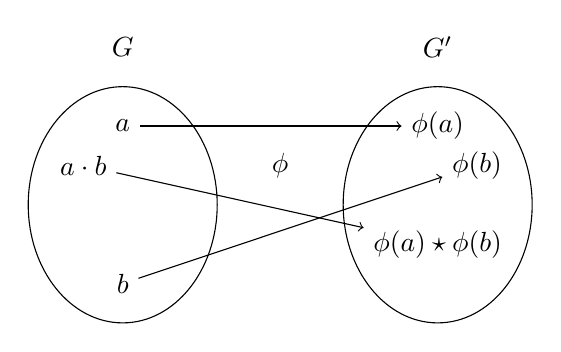
\begin{tikzpicture}
    \draw (-2,1.5) ellipse (1.2 and 1.5);
    \draw (2,1.5) ellipse (1.2 and 1.5);
    \node (v3) at (-2.5,2) {$a \cdot b$};
    \node (v1) at (-2,2.5) {$a$};
    \node (v5) at (-2,0.5) {$b$};
    \node (v2) at (2,2.5) {$\phi(a)$};
    \node (v4) at (2,1) {$\phi(a) \star \phi(b)$};
    \node (v6) at (2.5,2) {$\phi(b)$};
    \draw[->] (v1) edge (v2);
    \draw[->] (v3) edge (v4);
    \draw[->] (v5) edge (v6);
    \node at (-2,3.5) {$G$};
    \node at (2,3.5) {$G'$};
    \node at (0,2) {$\phi$};
  \end{tikzpicture}
  \caption{Isomorphismen lassen sich als Umbenennung der Gruppenelemente interpretieren.}
\end{figure}

Gibt es zwischen Gruppen $G$ und $G'$ einen Isomorphismus, so nennt man $G$ und $G'$ \emph{isomorph} und schreibt dies als $G \cong G'$.

Wir wollen uns die von verschiedenen Homomorphismen erzeugten Untergruppen genauer ansehen, da wir darüber Informationen über eine Gruppe erhalten können. Zwei Mengen sind hier von entscheidender Bedeutung:

\begin{definition}[Kern und Bild]
  Sei $\phi \colon G \rightarrow G'$ ein Gruppenhomomorphismus. Der \emph{Kern} von $\phi$ ist definiert als die Menge $\ker(\phi) = \left\{ g \in G \suchthat \phi(g)=e' \right\}$. Das \emph{Bild} von $\phi$ ist $\img(\phi) = \left\{ g' \in G' \suchthat \exists g \in G \text{ mit } \phi(g)=g'\right\}$.
\end{definition}

Der Kern und das Bild sollten selbst Untergruppen bilden, und das sind sie tatsächlich:

\begin{proposition}
  Ist $\phi \colon G \rightarrow G'$ ein Gruppenhomomorphismus, so gilt:
  \begin{enumerate}[label=\alph*)]
    \item $\ker(\phi) \leq G$
    \item $\img(\phi) \leq G'$
  \end{enumerate}
\end{proposition}

\begin{proof}
  \begin{enumerate}[label=\alph*)]
    \item Wir müssen zeigen, dass die Eigenschaften aus \reference{Definition}{def:algebra:untergruppe} gelten:
    \begin{enumerate}
      \item ist klar: $\phi(e)=e'$, also ist $e \in \ker(\phi)$.
      \item Angenommen, wir haben zwei Elemente $a,b \in \ker(\phi)$. Dann gilt die Gleichung $\phi(a \cdot b) = \phi(a) \star \phi(b) = e' \star e' = e'$, also ist auch $a \cdot b \in \ker(\phi)$.
      \item Sei $a \in \ker(\phi)$. Dann gilt $\phi(a^{-1}) = \phi(a)^{-1} = (e')^{-1} = e'$, somit ist auch $a^{-1} \in \ker(\phi)$.
    \end{enumerate}
    \item ist einfach, beziehungsweise analog zum ersten Teil.
  \end{enumerate}
\end{proof}

Auf der anderen Seite können wir auch Eigenschaften eines Homomorphismus aus dem Kern und Bild ablesen:

\begin{proposition}
  Ein Gruppenhomomorphismus $\phi \colon G \rightarrow G'$ ist genau dann injektiv, wenn $\ker(\phi) = \{e\}$.
\end{proposition}

\begin{proof}
  Wir zeigen die beiden Teile der Äquivalenz hintereinander.
  \begin{itemize}
    \item Wenn $\phi$ injektiv ist, so ist offensichtlich $\ker(\phi) = \{e\}$.
    \item Umgekehrt sei $\ker(\phi) = \{e\}$, und angenommen, es gäbe zwei Elemente $a,b \in G$ mit $a \neq b$ und $\phi(a) = \phi(b)$, also $\phi$ nicht injektiv. Dann gilt aber $a \cdot b^{-1} \neq e$ und $\phi(a\cdot b^{-1}) = \phi(a) \star \phi(b^{-1}) = \phi(a) \star \phi(b)^{-1} = \phi(a) \star \phi(a)^{-1} = e'$.
    Somit wäre $a \cdot b^{-1} \in \ker(\phi)$, was ein Widerspruch ist.
  \end{itemize}
\end{proof}

Schließlich wollen wir diesen Abschnitt mit einem interessanten Beispiel abschließen:

\begin{example}
  Wir wählen die zwei Gruppen $(\GL(n,\KK),\cdot)$ und $(\underbrace{\KK\setminus\{0\}}_{\eqqcolon \KK^\ast},\cdot)$, und betrachten die Abbildung
  \[\phi \colon \GL(n,\KK) \rightarrow \KK^\ast, \quad A \mapsto \det(A).\]

  Dann ist $\phi$ ein Gruppenhomomorphismus, weil nach Det.mult.satz gilt:\todowarning{Referenziere den DMS}
  \[\phi(A \cdot B) = \det(A \cdot B) = \det(A) \cdot \det(B) = \phi(A) \cdot \phi(B) \quad \forall A,B \in \GL(n,\KK).\]
\end{example}

\subsection{Links- und Rechtsnebenklassen}

\begin{definition}[Linksnebenklasse]
  Sei $G$ eine Gruppe und $H \leq G$. Eine Linksnebenklasse von $H$ in $G$ für ein $a \in G$ ist eine Teilmenge der Gestalt $a \cdot H = \left\{ a \cdot h \suchthat h \in H \right\}$.\todowarning{Bild}
\end{definition}

\begin{remark}
  Die Untergruppe $H$ selbst ist eine Linksnebenklasse, denn $H = 1 \cdot H$. Außerdem ist eine Linksnebenklasse von $H$ niemals leer, denn es gilt insbesondere $a \in aH$ mit $1 \in H$.
\end{remark}

\begin{lemma}[Linksnebenklassen]
  Für zwei Linksnebenklassen $aH$ und $bH$ von $H$ in $G$ sind äquivalent:
  \begin{enumerate}[label=\alph*)]
    \item $aH = bH$
    \item $aH \cap bH \neq \emptyset$
    \item $a \in bH$
    \item $b^{-1}a \in H$
  \end{enumerate}
\end{lemma}

\begin{proof}
  Wir werden den Ringschluss \emph{a)}$\Rightarrow$\emph{b)}$\Rightarrow$\emph{c)}$\Rightarrow$\emph{d)}$\Rightarrow$\emph{a)} zeigen.
  \begin{itemize}
    \item Die Implikation \emph{a)}$\Rightarrow$\emph{b)} ist klar.
    \item Für \emph{b)}$\Rightarrow$\emph{c)}, sei $c \in aH \cap bH$. Dann ist $c = a\cdot h_1$ und $c = b\cdot h_2$ für gewisse $h_1,h_2 \in H$ nach Definition der Linksnebenklassen. Also gilt $a\cdot h_1 = b\cdot h_2$, was allerdings impliziert, dass $a= b\cdot \underbrace{h_2\cdot h_1^{-1}}_{\in H} \in b \cdot H$ ist.
    \item Für \emph{c)}$\Rightarrow$\emph{d)} wissen wir, dass $a \in bH$ ist. Das heißt, $a = b\cdot h$ für ein gewisses $h \in H$. Aber dann ist wegen $b^{-1}\cdot a = h$ auch $b^{-1}\cdot a \in H$.
    \item Nun zur letzten Implikation \emph{d)}$\Rightarrow$\emph{a)}. Es gilt $b^{-1}\cdot a = h_0 \in H$, also $a=b\cdot h_0 \in bH$. Daher ist $a\cdot H = \left\{ a\cdot h \suchthat h \in H \right\} = \left\{ b\cdot h_0 \cdot h \suchthat h \in H \right\} \subseteq \left\{ b\cdot h' \suchthat h' \in H \right\} = b \cdot H$, kurz also $a\cdot H \subset b \cdot H$.
    Bleibt noch die umgekehrte Inklusion zu zeigen. Diese gilt jedoch nach dem gleichen Vorgehen, indem man benutzt, dass $(b^{-1}\cdot a)^{-1} = a^{-1} \cdot b \in H$ ist. Die Gleichheit gilt tatsächlich, denn offensichtlich ist $a^{-1}\cdot b \cdot b^{-1} \cdot a = 1$.
    Damit ist letztendlich $aH = bH$.
  \end{itemize}
\end{proof}

Das vorherige Lemma zeigt uns: Zwei Linksnebenklassen sind entweder gleich oder disjunkt.\todowarning{Bild} Jede Untergruppe $H \leq G$ induziert somit mittels Linksnebenklassen eine Partition von $G$.

\begin{theorem}[Mächtigkeit von Nebenklassen]

\end{theorem}

\begin{proof}

\end{proof}

\begin{remark}

\end{remark}}

% !TEX root = ../../MathLog.tex

\chapter{\IfLanguageName{english}{Number Theory}{Zahlentheorie}}


\part{\IfLanguageName{english}{Analysis and Geometry}{Analysis und Geometrie}}

% !TEX root = ../../MathLog.tex

\chapter{Analysis}

\IfLanguageName{english}{\todonote{stuff to translate here}}{Aus der Infinitesimalrechnung heraus hat sich bis heute die Analysis entwickelt, welche sich selbst wieder in viele Teilbereiche verzweigt. Daher wollen wir hier eine grundlegende Einführung wagen, allerdings auch ein paar fortgeschrittene und spezielle Themen behandeln.}

% !TEX root = ../../MathLog.tex

\chapter{\IfLanguageName{english}{Topology}{Topologie}}

\epigraph{Just got into topology. \\ That's some wild shit, yo.}{\textit{yourenothere1 on Reddit}}

% !TEX root = ../../MathLog.tex

\chapter{\IfLanguageName{english}{Geometry}{Geometrie}}

\IfLanguageName{english}{\todonote{translate here}}{Als eines der ältesten und umfassendsten Bereiche der Mathematik gilt die Geometrie. Daher lässt sie viele verschiedene Zugänge zu, beeinflusst aber auch selbst fast alle anderen Themengebiete in der Mathematik.

Eng verzahnt mit der Geometrie ist die Topologie, grob übersetzt auch \enquote{Lehre von Raum}.}

% !TEX root = ../../MathLog.tex

\chapter{\IfLanguageName{english}{Complex Analysis}{Komplexe Analysis (Funktionentheorie)}}

% !TEX root = ../../MathLog.tex

\chapter{\IfLanguageName{english}{Differential Geometry}{Differentialgeometrie}}


\part{\IfLanguageName{english}{Discrete and Algorithmic Mathematics}{Diskrete und algorithmische Mathematik}}

% !TEX root = ../../MathLog.tex

\chapter{\IfLanguageName{english}{Algorithmic und computer-oriented Mathematics}{Algorithmische und computerorientierte Mathematik}}

% !TEX root = ../../MathLog.tex

\chapter{\IfLanguageName{english}{Numerical Analysis}{Numerik}}

% !TEX root = ../../MathLog.tex

\chapter{\IfLanguageName{english}{Optimization}{Optimierung}}

\IfLanguageName{english}{\todonote{translate here} To get rid of the empty bibliography warning, we cite \textcite{Ziegl:Lectureson0/1}.}{Die Optimierung ist ein eher anwendungsorientierter Teilbereich der Mathematik. Trotz der Ausrichtung als algorithmisch motiviertes Gebiet sind viele vor allem geometrische Aspekte der Optimierung überraschend theoretisch. Für die algorithmische Seite wollen wir ebenfalls die Numerik betrachten.

Grundaufgabe der Optimierung ist meist, bestmögliche Parameter eines gegebenen, oftmals komplexen Systems zu finden.}

\section{\IfLanguageName{english}{Linear Optimization}{Lineare Optimierung}}

% !TEX root = ../../MathLog.tex
\chapter{\IfLanguageName{english}{Discrete Mathematics}{Diskrete Mathematik}}


\part{\IfLanguageName{english}{Probability Theory}{Wahrscheinlichkeitstheorie}}

% !TEX root = ../../MathLog.tex

\chapter{\IfLanguageName{english}{Probability Theory}{Wahrscheinlichkeitstheorie}}

\section{Martingales}


% !TEX root = ../MathLog.tex

\newbool{printSolutions} % declare a variable to print solutions
\booltrue{printSolutions} % set true with \booltrue, false with \boolfalse

% Write solutions in \ifbool{printSolutions}{ ... }{}

\part{\IfLanguageName{english}{Exercises}{Aufgaben}}

% !TEX root = ../../MathLog.tex
\chapter{\IfLanguageName{english}{Foundations of Mathematics}{Grundlagen der Mathematik}}


\section{\IfLanguageName{english}{Test exercise}{Testaufgabe}}

\IfLanguageName{english}{Exercise here}{Aufgabe hier}.

\ifbool{printSolutions}{
  \IfLanguageName{english}{Solution here}{Lösung hier}.
}{}

% !TEX root = ../../MathLog.tex
\chapter{\IfLanguageName{english}{Linear Algebra}{Lineare Algebra}}

% !TEX root = ../../MathLog.tex
\chapter{Algebra}

% !TEX root = ../../MathLog.tex

\chapter{\IfLanguageName{english}{Number Theory}{Zahlentheorie}}


% !TEX root = ../../MathLog.tex
\chapter{Analysis}

% !TEX root = ../../MathLog.tex
\chapter{\IfLanguageName{english}{Topology}{Topologie}}

% !TEX root = ../../MathLog.tex
\chapter{\IfLanguageName{english}{Geometry}{Geometrie}}

% !TEX root = ../../MathLog.tex

\chapter{\IfLanguageName{english}{Complex Analysis}{Komplexe Analysis (Funktionentheorie)}}

% !TEX root = ../../MathLog.tex

\chapter{\IfLanguageName{english}{Differential Geometry}{Differentialgeometrie}}


% !TEX root = ../../MathLog.tex

\chapter{\IfLanguageName{english}{Algorithmic und computer-oriented Mathematics}{Algorithmische und computerorientierte Mathematik}}

% !TEX root = ../../MathLog.tex

\chapter{\IfLanguageName{english}{Numerical Analysis}{Numerik}}

% !TEX root = ../../MathLog.tex
\chapter{\IfLanguageName{english}{Optimization}{Optimierung}}

% !TEX root = ../../MathLog.tex
\chapter{\IfLanguageName{english}{Discrete Mathematics}{Diskrete Mathematik}}


% !TEX root = ../../MathLog.tex

\chapter{\IfLanguageName{english}{Probability Theory}{Wahrscheinlichkeitstheorie}}

\section{Martingales}



%------------------------------------------------------------------------------
% CONTENT - APPENDICES
%------------------------------------------------------------------------------

\part{Appendices}
\appendix % Tell the documentclass that the appendices start here

% Include the appendices as separate files, inside the appendices file
% !TEX root = ../MathLog.tex

% !TEX root = ../MathLog.tex
\chapter{\IfLanguageName{english}{Computer Science}{Informatik}}



%------------------------------------------------------------------------------
% BIBLIOGRAPHY & INDEX
%------------------------------------------------------------------------------

%\nocite{*} % Cite all papers, regardless of citation
\printbibliography[heading=bibintoc]
\printindex

%------------------------------------------------------------------------------
\end{document}
